% !TeX encoding = UTF-8
% !TeX program = latexmk

\documentclass[xcolor=table,dvipsnames,svgnames,aspectratio=169,fontset=ubuntu]{ctexbeamer}
% Author: alick<alick9188@gmail.com>
% Author: justin <justin.w.xd@gmail.com>
% Author: Shengqi Chen <shengqi.chen@tuna.tsinghua.edu.cn>

% This file is modified from a solution template for:

% - Giving a talk on some subject.
% - The talk is between 15min and 45min long.
% - Style is ornate.

% Copyright 2004 by Till Tantau <tantau@users.sourceforge.net>.
%
% In principle, this file can be redistributed and/or modified under
% the terms of the GNU Public License, version 2.
%
% However, this file is supposed to be a template to be modified
% for your own needs. For this reason, if you use this file as a
% template and not specifically distribute it as part of a another
% package/program, I grant the extra permission to freely copy and
% modify this file as you see fit and even to delete this copyright
% notice.

\usepackage{tikz}

\graphicspath{{fig/}}

\mode<presentation>
{
  \usetheme{material}
  \renewcommand{\MaterialIcon}{tuna.pdf}
  \usefonttheme[onlymath]{serif}
  \setbeamercovered{transparent=5}
  \setbeamercolor*{structure}{fg=primaryD}
  \setbeamertemplate{itemize item}{\raise1.25pt\hbox{\tikz\draw[fill=fg] (0,0) circle (.3ex);}}
  \setbeamertemplate{itemize subitem}{\color{fg}\tiny\raise1.25pt\hbox{\donotcoloroutermaths$\blacktriangleright$}}
  \setbeamertemplate{itemize subsubitem}{\raise2.5pt\hbox{\tikz\draw[fill=fg] (0,0) rectangle (.7ex, .2ex);}}

  \setlength\leftmargini{1.4em}
  \setlength\leftmarginii{1.4em}
  \setlength\leftmarginiii{1.4em}
  \setbeamersize{description width=0.24cm}
}

\usepackage{mflogo} % for \MF, \MP
\usepackage{graphicx}
\usepackage{xspace}
\usepackage{amsmath}
\usepackage{unicode-math}
\usepackage{calligra}
\usepackage{fontspec}
\usepackage{ccicons}
\usepackage{hologo}
\usepackage{colortbl}
\usepackage{pstricks}
\usepackage{pst-node}
\usepackage{hyperxmp}
\usepackage{booktabs}
\usepackage{qrcode}
\usepackage{listings}
\usepackage{tipa}
\usepackage{xpinyin}
\usepackage{multicol}
\usepackage{datetime2}
\usepackage[normalem]{ulem}
\usepackage{fontawesome5}
\usepackage{hyperref}

\usetikzlibrary{arrows,intersections}
\usepackage[siunitx]{circuitikz}
\usepackage{animate}

\pdfstringdefDisableCommands{
  \let\\\relax
  \let\quad\relax
  \let\hspace\@gobble
}

% From thuthesis user guide
\makeatletter
\def\psRotation#1(#2,#3)#4{%
  \rput{#1}(#2,#3){%
    \psellipticarc[linewidth=.4pt]{->}(0,-0.1)(0.6,0.15){120}{70}
    \ifdim#1pt>\z@\rput[l]{*0}(0.675,0){#4}\else\rput[l](0.675,0){#4}\fi
  }%
}
\makeatother

% !TeX encoding = UTF-8
% !TeX program = latexmk
% !TeX root = latex-talk.tex

% fonts

% For tipa to work.
\defaultfontfeatures[TeX Gyre Termes]
{
  Extension      = .otf ,
  UprightFont    = texgyretermes-regular,
  BoldFont       = texgyretermes-bold,
  ItalicFont     = texgyretermes-italic,
  BoldItalicFont = texgyretermes-bolditalic,
}
\newfontfamily\useTIPAfont{TeX Gyre Termes}
\newfontfamily{\firamath}{FiraMath-Regular.otf}

% xeCJK conf setup
\renewcommand\CJKfamilydefault{\CJKsfdefault} % for slides

\IfFontExistsTF{Noto Sans CJK SC}{
    \setCJKsansfont{Noto Sans CJK SC}
}{} 
\IfFontExistsTF{Noto Sans Mono CJK SC}{
    \setCJKmonofont{Noto Sans Mono CJK SC}
}{}


% commands

\renewcommand{\TeX}{\hologo{TeX}}
\renewcommand{\LaTeX}{\hologo{LaTeX}}
\newcommand{\BibTeX}{\hologo{BibTeX}}
\newcommand{\XeTeX}{\hologo{XeTeX}}
\newcommand{\pdfTeX}{\hologo{pdfTeX}}
\newcommand{\LuaTeX}{\hologo{LuaTeX}}
\renewcommand{\CTeX}{C\TeX}
\newcommand{\MiKTeX}{\hologo{MiKTeX}}
\newcommand{\MacTeX}{Mac\hologo{TeX}}
\newcommand{\beamer}{\textsc{beamer}}
\newcommand{\XeLaTeX}{\hologo{Xe}\kern-.13em\LaTeX{}}
\newcommand{\pdfLaTeX}{pdf\LaTeX{}}
\newcommand{\LuaLaTeX}{Lua\LaTeX{}}

\def\TeXLive{\TeX{} Live\xspace}
\let\TL=\TeXLive
\newcommand{\TLVersion}{2024}
\newcommand{\ThuThesis}{\textsc{ThuThesis}\xspace}
\newcommand{\ThuThesisVersion}{7.6.0}
\newcommand{\ThuThesisDate}{2025/03/28}
\newcommand{\ThuThesisGuideVersion}{2025年3月}
\newcommand{\ThuThesisRepo}{tuna/thuthesis}
\newcommand{\ThuThesisLink}{https://github.com/\ThuThesisRepo}

\newcommand{\surveylink}{\relax}
\newcommand{\thudownloadlink}{https://stu.cs.tsinghua.edu.cn/\~harry/latex-talk.pdf}
\newcommand{\githubrepo}{tuna/thulib-latex-talk}
\newcommand{\githublink}{https://github.com/\githubrepo}

\newcommand{\printcurrenttoc}{
  \begin{frame}<beamer>{目录}
    \tableofcontents[currentsection,currentsubsection]
  \end{frame}
}


\newcommand\link[1]{\href{#1}{\faLink}}
\newcommand\pkg[1]{\texttt{#1}}

% From thuthesis user guide.
\def\cmd#1{\texttt{\color{DarkBlue}\footnotesize $\backslash$#1}}
\def\env#1{\texttt{\color{DarkBlue}\footnotesize #1}}
\def\cmdxmp#1#2#3{\small{\texttt{\color{DarkBlue}$\backslash$#1}\{#2\}\hspace{1em}\\ $\Rightarrow$\hspace{1em} {#3}\par\vskip1em}}


\lstset{
  language=[LaTeX]TeX,
  basicstyle=\ttfamily\footnotesize,
  tabsize=2,
  keywordstyle=\bfseries\ttfamily\color{primaryD},
  commentstyle=\sl\ttfamily\color[RGB]{100,100,100},
  stringstyle=\ttfamily\color[RGB]{50,50,50},
  extendedchars=true,
  breaklines=true,
}
\lstdefinestyle{style@inline}{
  basicstyle   = \ttfamily,
  keepspaces   = true
}
\lstMakeShortInline[style=style@inline]|

\title{如何使用 \LaTeX 排版论文}

\author[陈晟祺]{\vspace{1em} 陈晟祺\\ \texttt{shengqi.chen@tuna.tsinghua.edu.cn}}
\institute{清华大学 TUNA 协会}
\date[清华大学图书馆培训讲座]{\the\year 年 \the\month 月}
\subject{LaTeX, 论文排版, ThuThesis}

% Delete this, if you do not want the table of contents to pop up at
% the beginning of each subsection:
\AtBeginSubsection[]{\printcurrenttoc}

\hypersetup{
  pdfsubject = {清华大学图书馆培训讲座},
  pdfauthor = {Shengqi Chen, Justin Wong, Alick Zhao},
  pdfcopyright = {Copyright (C) 2015-\the\year by Alick Zhao, Justin Wong and Shengqi Chen. Licensed under CC-BY-SA 4.0. Some rights reserved.},
  pdflicenseurl = {http://creativecommons.org/licenses/by-sa/4.0/},
  unicode            = true,
  psdextra           = true,
  pdfdisplaydoctitle = true
}

\logo{\includegraphics[height=.15\textheight]{libicon.pdf}}

\begin{document}

\begin{frame}
  \titlepage
\end{frame}


\begin{frame}{关于}
  \begin{columns}[c]
    \begin{column}{.7\textwidth}
      \begin{itemize}
        \item 最后更新:\texttt{\DTMnow}
        \item 本幻灯片源码:
          \begin{itemize}
            \item \url{\githublink}
          \end{itemize}
        \item 本幻灯片参考:
          \begin{itemize}
            \item \url{http://github.com/alick/fad-texlive-talk}
            \item \url{https://github.com/stone-zeng/latex-talk}
            \item \ThuThesis{} 使用示例文档 v\ThuThesisVersion
          \end{itemize}
        \item 本幻灯片下载(实时更新):
          \begin{itemize}
            \item GitHub Releases \link{\githublink/releases}
            \item 校内镜像 \link{\thudownloadlink}
          \end{itemize}
        \item 许可证:CC BY-SA 4.0 Unported \ccbysa
      \end{itemize}
    \end{column}
    \begin{column}{.3\textwidth}
      \qrcode[hyperlink, height=4cm]{\thudownloadlink}
    \end{column}
  \end{columns}
\end{frame}


\begin{frame}{目录}
  \tableofcontents
  % You might wish to add the option [pausesections]
\end{frame}


% !TeX encoding = UTF-8
% !TeX program = latexmk
% !TeX root = ../latex-talk.tex

\section{简介}

\subsection{\TeX 与 \LaTeX}

\begin{frame}[fragile]{\TeX 与 \LaTeX}
  \begin{columns}[T]
    \column{.8\textwidth}
    \begin{itemize}
      \item \TeX: $\tau\varepsilon\chi$ (\textipa{/'tEx/},
        \textipa{/'tEk/})
        \begin{itemize}
          \item 生成精美图书的排版系统
          \item 最初由 高德纳 (Donald E.~Knuth) 于 1978 年开发
          \item 发音接近“泰赫”,而非“泰克斯”,
            Knuth 对此有\xpinyin{强}{\useTIPAfont qiang3}迫症
          \item 每 7 年发布新版,最新版本为 \TeX\ 3.141592653(2021年1月)\link{https://tex.stackexchange.com/questions/581118/whats-new-in-tex-version-3-141592653}
          \item 漂亮、美观、稳定、通用
          \item 尤其擅长数学公式排版
        \end{itemize}
      \item \LaTeX\ (\textipa{/'la:tEx/}, \textipa{/'leItEk/})
        \begin{itemize}
          \item Leslie Lamport 开发的一种 \TeX{} 格式
          \item 在 \TeX 的基础上提供宏包, 降低使用门槛
          \item 极其丰富的宏包,提供扩展功能
          \item 广泛用于学术界,期刊会议论文模板
          \item 大学学位论文模板,如 \ThuThesis
        \end{itemize}
    \end{itemize}
    \column{.2\textwidth}
    %\vspace*{5mm}
    \includegraphics[width=\textwidth]{Knuth.jpg}

    %\vspace*{5mm}
    \includegraphics[width=\textwidth]{Lamport.jpg}

  \end{columns}
\end{frame}

\begin{frame}{和 Word 对比}
  注:术业有专攻,评价需客观
  \begin{table}[h]
    \centering
    \rowcolors[]{1}{primaryL}{primaryL!40}
    \begin{tabular}{c|c}
      Microsoft\textsuperscript{\textregistered}  Word & \LaTeX \\
      \hline
      字处理工具 & 专业排版软件 \\
      容易上手,简单直观 & 容易上手 \\
      所见即所得 & 所见即所想,所想即所得 \\
      高级功能不易掌握 & 进阶难,但一般用不到 \\
      处理长文档需要丰富经验 & 和短文档处理基本无异 \\
      花费大量时间调格式 & 无需担心格式,专心作者内容 \\
      公式排版差强人意 & 尤其擅长公式排版 \\
      二进制格式,兼容性差 & 文本文件,易读、稳定 \\
      付费商业许可 & 自由免费使用 \\
    \end{tabular}
  \end{table}
\end{frame}

\begin{frame}{\TeX{}排版举例:公式}
  \begin{exampleblock}{无编号公式}
    \begin{equation*}
      \mathcal{F}(\xi)=\int_{-\infty}^{\infty} f(x)\mathrm{e}^{-\mathrm{j}2\pi \xi x}\,\mathrm{d}x
    \end{equation*}
  \end{exampleblock}
  \begin{exampleblock}{多行多列公式}
    % Taken from Mathmode.tex
    \begin{align}
      y & =d & z & =1\\
      y & =cx+d & z & =x+1\\
      y_{12} & =bx^{2}+cx+d & z & =x^{2}+x+1\nonumber \\
      y(x) & =ax^{3}+bx^{2}+cx+d & z & =x^{3}+x^{2}+x+1
    \end{align}
  \end{exampleblock}
\end{frame}

\begin{frame}{\TeX{}排版举例:公式}
  \begin{exampleblock}{编号多行公式}
    % Taken from Mathmode.tex
    \begin{multline}
    A=\lim_{n\rightarrow\infty}\Delta x\left(a^{2}+\left(a^{2}+2a\Delta x+\left(\Delta x\right)^{2}\right)\right.\label{eq:reset}\\
    +\left(a^{2}+2\cdot2a\Delta x+2^{2}\left(\Delta x\right)^{2}\right)\\
    +\left(a^{2}+2\cdot3a\Delta x+3^{2}\left(\Delta x\right)^{2}\right)\\
    +\ldots\\
    \left.+\left(a^{2}+2\cdot(n-1)a\Delta x+(n-1)^{2}\left(\Delta x\right)^{2}\right)\right)\\
    =\frac{1}{3}\left(b^{3}-a^{3}\right)
  \end{multline}
\end{exampleblock}
\end{frame}

\begin{frame}{\TeX{}排版举例:图形与图表}
  \begin{minipage}[c]{0.3\linewidth}
    % !TeX encoding = UTF-8
% !TeX program = latexmk
% !TeX root = ../../latex-talk.tex

% adapted from https://texample.net/tikz/examples/linear-regression/

\begin{tikzpicture}[
    % thick,
    >=stealth',
    dot/.style = {
      draw,
      fill = white,
      circle,
      inner sep = 0pt,
      minimum size = 4pt
    },
    font=\rmfamily\footnotesize,
    scale=0.6,
    every node/.style={scale=0.6}
  ]
  \coordinate (O) at (0,0);
  \draw[->] (-0.3,0) -- (8,0) coordinate[label = {below:$x$}] (xmax);
  \draw[->] (0,-0.3) -- (0,5) coordinate[label = {right:$f(x)$}] (ymax);
  \path[name path=x] (0.3,0.5) -- (6.7,4.7);
  \path[name path=y] plot[smooth] coordinates {(-0.3,2) (2,1.5) (4,2.8) (6,5)};
  \scope[name intersections = {of = x and y, name = i}]
    \fill[gray!20] (i-1) -- (i-2 |- i-1) -- (i-2) -- cycle;
    \draw      (0.3,0.5) -- (6.7,4.7) node[pos=0.8, below right] {Secant line};
    \draw[red] plot[smooth] coordinates {(-0.3,2) (2,1.5) (4,2.8) (6,5)};
    \draw (i-1) node[dot, label = {above:$P$}] (i-1) {} -- node[left]
      {$f(x_0)$} (i-1 |- O) node[dot, label = {below:$x_0$}] {};
    \path (i-2) node[dot, label = {above:$Q$}] (i-2) {} -- (i-2 |- i-1)
      node[dot] (i-12) {};
    \draw           (i-12) -- (i-12 |- O) node[dot,
                              label = {below:$x_0 + \varepsilon$}] {};
    \draw[blue, <->] (i-2) -- node[right] {$f(x_0 + \varepsilon) - f(x_0)$}
                              (i-12);
    \draw[blue, <->] (i-1) -- node[below] {$\varepsilon$} (i-12);
    \path       (i-1 |- O) -- node[below] {$\varepsilon$} (i-2 |- O);
    \draw[gray]      (i-2) -- (i-2 -| xmax);
    \draw[gray, <->] ([xshift = -0.5cm]i-2 -| xmax) -- node[fill = white]
      {$f(x_0 + \varepsilon)$}  ([xshift = -0.5cm]xmax);
  \endscope
\end{tikzpicture}

  \end{minipage}\hspace{1cm}
  \begin{minipage}[t]{0.5\linewidth}
    \centering
    \begin{circuitikz}[scale=0.8,every node/.style={scale=0.6},font=\rmfamily]\draw
      (0,0) node[ground] {}
          to[V=$e(t)$, *-*] (0,2) to[C=4<\nano\farad>] (2,2)
          to[R, l_=.25<\kilo\ohm>, *-*] (2,0)
      (2,2) to[R=1<\kilo\ohm>] (4,2)
          to[C, l_=2<\nano\farad>, *-*] (4,0)
      (5,0) to[I, i_=$a(t)$, -*] (5,2) -- (4,2)
      (0,0) -- (5,0)
      (0,2) -- (0,3) to[L, l=2<\milli\henry>] (5,3) -- (5,2)
      {[anchor=south east] (0,2) node {1} (2,2) node {2} (4,2) node {3}}
      ;
    \end{circuitikz}
    % \hspace{2cm}
    \begin{figure}[h]
      \centering
      % !TeX encoding = UTF-8
% !TeX program = latexmk
% !TeX root = ../../latex-talk.tex

% adapted from https://texample.net/tikz/examples/animated-distributions/

\newcounter{tikzdistcnt}
\setcounter{tikzdistcnt}{0}

\newcommand{\distpic}[3]{

    % Now draw the lower distribution showing the effect size:
    \begin{scope}
    % Shade the "reject H0" region red
    \fill[red!30] (0.658,0)  -- plot[id=f3\thetikzdistcnt,domain=0.658:3,samples=50]
        function {exp(-(x-#1)*(x-#1)*0.5/0.16)} --
        (3,0) -- cycle;
        % Shade the "accept H0" region blue
    \fill[blue!30] (-2,0) -- plot[id=f4\thetikzdistcnt,domain=-2:0.658,samples=50]
        function {exp(-(x-#1)*(x-#1)*0.5/0.16)} --
        (0.658,0) -- cycle;

        % Draw the shifted normal distribution:
    \draw[blue!50!black,smooth,thick] plot[id=f1\thetikzdistcnt,domain=-2:3,samples=50]
            function {exp(-(x-#1)*(x-#1)*0.5/0.16)};

        % Draw the x-axis and put in some ticks and tick labels
    \draw[->,black] (-2.2,0) -- (3.2,0);
    \foreach \x in {-2,-1,0,1,2,3}
            \draw (\x,0) -- (\x,-0.1) node[below] {$\x$};

        % Draw and label the critical region boundary
    \draw[red!50!black,very thick] (0.658,0) node[below,yshift=-0.5cm] {0.658}
        -- (0.658,1.0);
    \draw[red!50!black,very thick,->] (0.688,0.7) -- (2.7,0.7)
        node[anchor=south west] {Reject  $H_0$};
    \draw[red!50!black,very thick,->] (0.628,0.7) -- (-0.5,0.7)
        node[anchor=south]{\parbox{1.5cm}{\raggedright Fail to reject $H_0$}};

    % Add a label to the lower picture, when the alternative hypothesis is true:
    \draw (-3,1) node[above,draw,fill=green!30] {$H_a$ is true:};

        % Add labels showing the statistical power and the Type II error rate:
    \draw[<-,thick] (1.5,0.1) -- (3,0.2) node[anchor=south west]
        {Power = #2};
    \draw[<-,thick] (0.4,0.1) -- (-1,0.2) node[left,yshift=0.3cm]
        {\begin{tabular}{l}
        $\beta$ = {#3} \\ (Type II error rate) \end{tabular}};
    \end{scope}
}

\begin{animateinline}[
  autoplay,
  loop,
  begin={
    \begin{tikzpicture}[
      scale=1,
      font=\rmfamily\scriptsize,
      every node/.style={scale=1,font=\rmfamily\scriptsize}
  ]},
  end={\stepcounter{tikzdistcnt}\end{tikzpicture}}
]{3}
  \distpic{0.5}{.346}{.654}\newframe
  \distpic{0.7}{.542}{.458}\newframe
  \distpic{0.9}{.727}{.273}\newframe
  \distpic{1.1}{.865}{.135}\newframe
  \distpic{1.3}{.946}{.054}\newframe
  \distpic{1.5}{.982}{.018}\newframe
  \distpic{1.7}{.995}{.005}\newframe
  \distpic{1.9}{.999}{.001}
\end{animateinline}

    \end{figure}
  \end{minipage}
\end{frame}

\begin{frame}{\TeX{}排版举例:文档}
  \begin{columns}
    \begin{column}{.45\textwidth}
      \begin{figure}[h]
        \centering
        \includegraphics[width=.8\textwidth]{references.pdf}
      \end{figure}
    \end{column}
    \begin{column}{.45\textwidth}
      \begin{figure}[h]
        \centering
        \includegraphics[width=.8\textwidth]{shapepar.pdf}
      \end{figure}
    \end{column}
  \end{columns}
\end{frame}

\begin{frame}{\TeX{}排版举例:幻灯片}
  \begin{columns}
    \begin{column}{.45\textwidth}
      \begin{figure}[h]
        \centering
        \includegraphics[width=\textwidth]{slides-powerdot.pdf}
      \end{figure}
    \end{column}
    \begin{column}{.45\textwidth}
      \begin{figure}[h]
        \centering
        \includegraphics[width=\textwidth]{slides-beamer.pdf}
      \end{figure}
    \end{column}
  \end{columns}
\end{frame}

\subsection{安装}

\begin{frame}{如何安装 \hologo{(La)TeX}?}
  \begin{itemize}
    \item \TeX{}发行版(Distro)
      \begin{itemize}
        \item \TeX{}实用工具大集合:引擎、宏包、文档等
        \item 常见\TeX{}发行版:
          \alert{\TL{} / \MacTeX}, \CTeX, \MiKTeX
      \end{itemize}
    \item \TL
      \begin{itemize}
        \item 跨平台:Windows、Linux、macOS(二次打包后称为 \MacTeX)
        \item 每年四月左右发布以年份命名的新版本,当前为 \TL \TLVersion
      \end{itemize}
    \item \MiKTeX
      \begin{itemize}
        \item 最早专为 Windows 开发,现亦有 Linux 和 macOS 版本
        \item 由 Christian Schenk 个人维护,轻量安装,滚动更新
      \end{itemize}
    \item \CTeX
      \begin{itemize}
        \item 中科院吴凌云研究员基于 \MiKTeX 开发,并打包 WinEdt 等多种工具
        \item 在早期极大地方便了 Windows 上的中文 \TeX 用户
        \item 2012-2022 年暂停开发,目前已经恢复更新
      \end{itemize}
  \end{itemize}
\end{frame}

\begin{frame}[fragile]
  \frametitle{下载 \TL}
  \begin{itemize}
    \item 注意!
      \begin{itemize}
        \item Windows 下不要放在带有中文的路径中
      \end{itemize}
    \item 离线安装镜像(约 6GB 大小)
      \begin{itemize}
        \item {\footnotesize
          \url{https://mirrors.tuna.tsinghua.edu.cn/CTAN/systems/texlive/Images/texlive.iso}}
      \end{itemize}
    \item 在线安装包 (和相应的校验文件,以 .sha256 结尾)
      \begin{itemize} % several mirror url
        \item {\footnotesize
          \url{https://mirrors.tuna.tsinghua.edu.cn/CTAN/systems/texlive/tlnet/}
        }
        \item 更多可见 \url{http://mirror.ctan.org/README.mirrors}
      \end{itemize}

    \item 可选步骤:校验安装包
      \begin{lstlisting}[language=tex]
LANG=C sha256sum --check install-tl-unx.tar.gz.sha256
install-tl-unx.tar.gz: OK
      \end{lstlisting}

  \end{itemize}
\end{frame}

\begin{frame}[fragile]
  \frametitle{安装 \TL}
  \begin{itemize}
    \item Windows
      \begin{itemize}
        \item 解压或挂载下载的 ISO,运行 |install-tl-windows.bat|
        \item 切换默认仓库为国内镜像(如 TUNA)可加速今后升级
      \end{itemize}
    \item macOS
      \begin{itemize}
        \item 需要下载独立的安装包 \link{https://mirrors.tuna.tsinghua.edu.cn/CTAN/systems/mac/mactex/MacTeX.pkg}
      \end{itemize}
    \item Linux
      \begin{itemize}
        \item 不推荐从发行版仓库直接安装(更新缓慢)
        \item 图形安装界面需要 Perl Tk 模块
          \begin{lstlisting}
yum install perl-Tk 或 apt-get install perl-tk
sudo mkdir /usr/local/texlive
sudo chown yourname:yourname /usr/local/texlive
./install-tl -gui -repository \
  https://mirrors.tuna.tsinghua.edu.cn/CTAN/systems/texlive/tlnet/
        \end{lstlisting}
      \end{itemize}
\end{itemize}
\end{frame}

\begin{frame}[fragile]
  \frametitle{\TL 安装后配置(仅 Linux)}
  \begin{itemize}
    \item
      添加环境变量到 shell 配置(如 \nolinkurl{~/.bashrc}):
      \begin{lstlisting}[language=bash]
export PATH=/usr/local/texlive/current/bin/x86_64-linux:$PATH
export MANPATH=/usr/local/texlive/current/texmf/doc/man:$MANPATH
export INFOPATH=/usr/local/texlive/current/texmf/doc/info:$INFOPATH
      \end{lstlisting}
  \item
    阅读 \TeXLive 指南中文版 |texlive-zh-cn.pdf|,
    关注第 3.4 节:
      \begin{lstlisting}[basicstyle=\ttfamily]
texdoc texlive-zh
      \end{lstlisting}
  \end{itemize}
\end{frame}

\begin{frame}[fragile]
  \frametitle{安装后配置(仅 Linux)}
  \begin{itemize}
  \item
    \XeTeX\ 系统字体配置
    \begin{lstlisting}[language=bash]
cp /usr/local/texlive/current/texmf-var/fonts/conf/texlive-fontconfig.conf \
  /etc/fonts/conf.d/09-texlive.conf
fc-cache -fsv
    \end{lstlisting}
  \item 安装一个 dummy package,让系统的包管理器知道 \TL 已经装过了
    \begin{itemize}
      \item Arch Linux 用户装 AUR 里的 \verb|texlive-dummy|
      \item Debian/Ubuntu 用户参照手册做一个包即可 \link{https://www.tug.org/texlive/debian.html\#vanilla}
      \item Fedora 用户可以直接下载 \link{https://copr.fedoraproject.org/coprs/fatka/texlive-dummy/}
    \end{itemize}
  \item 部分教程可参考:
    \link{http://zhuanlan.zhihu.com/LaTeX/20069414}
    \link{https://stone-zeng.github.io/2018-05-13-install-texlive-ubuntu/}
  \end{itemize}
\end{frame}

\begin{frame}{编辑器配置}
  \begin{itemize}
    \item \TeX{}编辑器
      \begin{itemize}
        \item 专用编辑器:TeXworks、\alert{TeXStudio}、TeXmaker、WinEdt 等
        \item 通用编辑器(安装 \LaTeX{} 插件):Vim、Emacs、\alert{VS Code}、Sublime、Atom 等
      \end{itemize}
  \end{itemize}
  \begin{exampleblock}{TeXStudio 配置}
    \begin{itemize}
      \item Options -> Configure TeXstudio
        \begin{itemize}
          \item Build:Default Compiler 选择 \XeLaTeX{}
          \item 搜索框输入 Line Number -> Adv. Editor -> 打开行号
        \end{itemize}
    \end{itemize}
  \end{exampleblock}
\end{frame}


\begin{frame}[fragile]
  \frametitle{使用在线协作平台}
  \begin{itemize}
    \item 通过在线平台编辑、编译
      \begin{itemize}
        \item Overleaf:\url{https://www.overleaf.com/}
        \item TeXPage:\url{https://www.texpage.com/}
        \item 清华大学 Overleaf 服务(校园网):\url{https://overleaf.tsinghua.edu.cn/}
      \end{itemize}
    \item 免去安装、升级等一系列烦恼
    \item 可以多人协作
    \item 支持中文,可能需要自己上传字体
      \begin{itemize}
        \item 可直接使用 \pkg{ctex} 宏集和 \pkg{thuthesis} 文档模板,中文排版体验较好
        \item TeXPage、清华 Overleaf 均内置较多中文字体
      \end{itemize}
    \item 容量有一定限制
  \end{itemize}
\end{frame}


\begin{frame}[fragile]{后期安装或更新宏包}
  \begin{exampleblock}{很多时候需要自己安装宏包}
    % \vspace*{-3mm}
    \begin{itemize}
      \item 发行版没有预装
      \item 宏包需要更新(\TL 升级间隔的尴尬时期,或者宏包有重大变化)
    \end{itemize}
  \end{exampleblock}
  % \vspace*{-3mm}
  \begin{exampleblock}{\TL 或 \MacTeX}
    % \vspace*{-3mm}
    \begin{itemize}
      \item (Windows)开始菜单里找 TeX Live Manager
      \item 设置仓库地址 |tlmgr option repository| {\footnotesize\ttfamily
        https://mirrors.tuna.tsinghua.edu.cn/CTAN/systems/texlive/tlnet}
      \item |tlmgr install <pkgname>| 安装、 |tlmgr update --self --all| 全部更新
    \end{itemize}
  \end{exampleblock}
  % \vspace*{-3mm}
  \begin{exampleblock}{\CTeX 或 \MiKTeX}
    % \vspace*{-3mm}
    \begin{itemize}
      \item 开始菜单里找 CTeX / MiKTeX -> Package Manager
      \item 在 WinEdt 里 MiKTeX Options -> Packages
    \end{itemize}
  \end{exampleblock}
\end{frame}

%\begin{frame}
%\frametitle{网络安装后测试}
%\framesubtitle{English 测试}

%\begin{exampleblock}{使用已安装的示例文件}
%\begin{itemize}
%\item \texttt{latex sample2e.tex \#} .tex $\rightarrow$ .dvi (device independent)

%\texttt{xdvi sample2e.dvi \#} also try dvipdf sample2e.dvi
%\item try \texttt{pdflatex sample2e} directly
%\item \texttt{xetex opentype-info.tex \#} test of xetex's OpenType support
%\end{itemize}

%\end{exampleblock}
%\end{frame}

\begin{frame}[fragile]
  \frametitle{安装后测试}

  \begin{itemize}
    \item 编辑 \texttt{hello.tex} (Windows 下不要用中文文件名,注意
      \LaTeX{} 对文件名大小写敏感)
      \lstset{language=[LaTeX]TeX}
      \begin{card} \begin{lstlisting}[basicstyle=\ttfamily]
\documentclass{ctexart} % 使用中文适配的 article 文档类
\begin{document}
\TeX{}你好!
\end{document}
        \end{lstlisting}\end{card}
      \begin{itemize}
        \item Windows 下缺省使用中易字体
        \item Linux、macOS 下需要注意字体(参见 \pkg{ctex} 文档)
      \end{itemize}
    \item 使用 \XeLaTeX{} 引擎编译,得到 PDF 文档
      \begin{center}
        \fbox{\textrm \TeX{}\songti 你好!}
      \end{center}
  \end{itemize}
\end{frame}

%%% vim: set ts=2 sts=2 sw=2 isk+=\: et tw=80 cc=+1 formatoptions+=mM:

\include{content/02.basis}
% !TeX encoding = UTF-8
% !TeX program = latexmk
% !TeX root = ../latex-talk.tex

\section{学位论文排版}
\subsection{\ThuThesis 清华大学学位论文模板}

\begin{frame}{\ThuThesis}
  \framesubtitle{清华大学学位论文 \LaTeX{} 模板}
  \begin{itemize}
  \item 最早由王磊于 2004年4月发布,2005 年薛瑞尼接手维护,2018年起李泽平为主力开发者,2020年起由TUNA维护
  \item 最新正式版:\ThuThesisVersion\ (\ThuThesisDate)
  \item 全面支持最新的本科、研究生\footnote{更新到\ThuThesisGuideVersion{}发布的《清华大学研究生学位论文写作指南》,并支持若干院系的特殊要求}、博士后论文/报告格式,获研究生院官方推荐 \link{https://info2021.tsinghua.edu.cn/f/info/xxfb_fg/xnzx/template/detail?xxid=fa880bdf60102a29fbe3c31f36b76c7e}
  \end{itemize}
  \begin{figure}[htbp]
    \centering
    
\includegraphics[height=.4\textheight]{cover-bachelor-crop.pdf}\hfill
    
\includegraphics[height=.4\textheight]{cover-master-crop.pdf}\hfill
    
\includegraphics[height=.4\textheight]{cover-doctor-crop.pdf}\hfill
    
\includegraphics[height=.4\textheight]{cover-postdoc-crop.pdf}
  \end{figure}
\end{frame}

\begin{frame}[fragile]{手动安装\ThuThesis{}}
      \begin{columns}
        \begin{column}{.75\textwidth}
  \begin{itemize}
    \item 下载最新正式版(推荐)
      \begin{itemize}
        \item CTAN 官方 \link{http://mirrors.ctan.org/macros/latex/contrib/thuthesis.zip}(发行版可使用自带更新机制)
        \item GitHub Releases \link{\ThuThesisLink/releases} 或 TUNA 镜像 \link{https://mirrors.tuna.tsinghua.edu.cn/github-release/\ThuThesisRepo/}
      \end{itemize}
    \item 从 CI 下载最新开发版(高级 / 想尝鲜 / 着急的用户)
      \begin{itemize}
        \item \url{\ThuThesisLink}
        \item 点击 master 分支的小绿勾——点击“build”一项旁边的“Details”链接进入 CI 详情
        \item 点击左侧边栏“Summary”——滚动页面到最底下,从“Artifacts”中选择 |build-snapshot-release| 下载
        \item 解压下载的 ZIP 文件,得到 |dist/thuthesis-v*.zip|
      \end{itemize}
  \end{itemize}
        \end{column}
        \begin{column}{.25\textwidth}
          \begin{figure}[htbp]
            \centering
            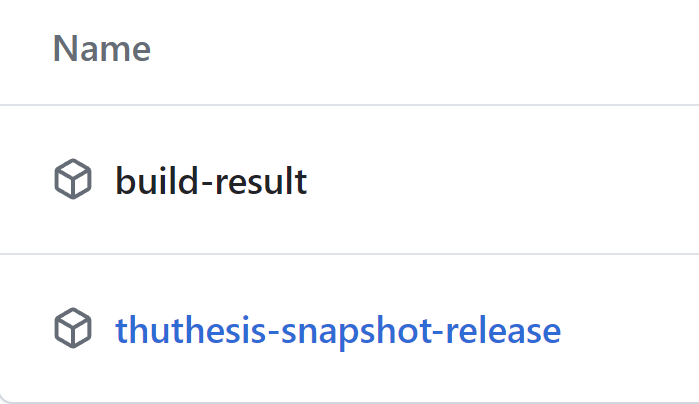
\includegraphics[width=.95\textwidth]{thuthesis-download.png}
          \end{figure}
        \end{column}
      \end{columns}
  \begin{itemize}
    \item 编译与安装
      \begin{itemize}
        \item 解压缩 |thuthesis-v*.zip| 后\textbf{先看文档} |README.md|
        \item 模板文档类:|thuthesis.cls| 已经编译好,无需额外操作
        \item 论文示例:|make thesis| 编译 |thuthesis-example.tex| $\Rightarrow$
        |thuthesis-example.pdf|
        \item 用户手册:|make doc| 编译 |thuthesis.dtx| $\Rightarrow$
          |thuthesis.pdf|
        \item 更多用法可参考附带的 |Makefile|
      \end{itemize}
  \end{itemize}
\end{frame}

\begin{frame}[fragile]{模板选项}
\begin{description}
\item[degree] 指定学位类型(本科/硕士/博士/博后)
  \begin{lstlisting}[basicstyle=\ttfamily]
\documentclass[degree=bachelor]{thuthesis}
  \end{lstlisting}
\item[degree-type] 指定学位选项(专硕/学硕格式不同)
  \begin{lstlisting}[basicstyle=\ttfamily]
\documentclass[degree=master,degree-type=professional]{thuthesis}
  \end{lstlisting}
\item[fontset] 指定字体(推荐使用 |windows|,详见模板文档说明)
  \begin{lstlisting}[basicstyle=\ttfamily]
\documentclass[degree=doctor,fontset=windows]{thuthesis}
  \end{lstlisting}
\end{description}
\end{frame}

\begin{frame}[fragile]{封面}
  使用 |\thusetup| 命令指定论文各类选项:
  \begin{table}[h]
    \centering
\footnotesize
  \begin{tabular}{lll} \toprule
    命令作用 & 中文对应选项 & 英文对应选项 \\ \midrule
  论文标题 & |title| & |title*| \\
  作者姓名&  |author| &|author*|\\
  申请学位类型 & |degree-category|&|degree-category*|\\
  院系名称 & |department| & |department*|\\
  学科名称 & |discipline| & |discipline*|\\
  专业领域 & |professional-field| & |professional-field*|\\
  导师 & |supervisor| & |supervisor*|\\
  副导师 & |associate-supervisor| & |associate-supervisor*|\\
  联合导师 & |joint-supervisor| & |joint-supervisor*|\\
  日期 & \multicolumn{2}{c}{\texttt{date}}\\
  密级 & \multicolumn{2}{c}{\texttt{secret-year, secret-level}}\\
  语言(环境名称等) & \multicolumn{2}{c}{\texttt{language}} \\ 
  博后专用 & \multicolumn{2}{c}{\texttt{clc, udc, id, ...}} \\ \bottomrule
  \end{tabular}
  \end{table}
\end{frame}

\begin{frame}[fragile]{数学}
  \begin{itemize}
    \item 公式示例:\nolinkurl{data/chap01.tex}
    \item \ThuThesis{} 定义了常用的数学环境(需要手工引入 |amsthm| 宏包):
      \begin{table}[h]
        \centering
        \footnotesize
\begin{tabular}{*{7}{l}}\toprule
  axiom & theorem & definition & proposition & lemma & conjecture &\\
  公理 & 定理 & 定义 & 命题 & 引理 & 猜想 &\\\midrule
  proof & corollary & example & exercise & assumption & remark & problem \\
  证明 & 推论 & 例子& 练习 & 假设 & 注释 & 问题\\\bottomrule
\end{tabular}
      \end{table}
      \item \ThuThesis{} 使用 \pkg{unicode-math} 进行数学输入(\ref{frame:unicode-math} 页),注意与传统方式的区别
  \end{itemize}
\end{frame}

\begin{frame}[fragile]{参考文献}
  \begin{itemize}
    \item 使用 \BibTeX 和 \pkg{natbib} 宏包
      \begin{itemize}
        \item 本科生文献翻译/阅读报告的参考文献与正文独立
        \item 推荐使用 |latexmk| 编译以保证参考文献生成正确
      \end{itemize}
    \item 模板支持两种引用方式:
      \begin{itemize}
        \item 顺序编码制(默认),其中包含两种模式:
        \begin{itemize}
          \item 上标模式:如“在许多文献\textsuperscript{[12-13]}中……”
          \begin{lstlisting}[basicstyle=\ttfamily]
    \cite{key12, key13}
          \end{lstlisting}
        \item 正文模式:如“文献~[14] 证明了……”
          \begin{lstlisting}[basicstyle=\ttfamily]
    \inlinecite{key14}
          \end{lstlisting}
        \end{itemize}
        \item 著者-出版年制,包括两种引用模式(\cmd{citep}, \cmd{citet})
      \end{itemize}
    \end{itemize}
\end{frame}

% \begin{frame}{作图}
%   \begin{columns}[c]
%     \begin{column}{.5\textwidth}
%   \begin{itemize}
%   \item 矢量图 eps, ps, pdf
%     \begin{itemize}
%     \item \MP, pstricks, pgf $\ldots$
%     \item Xfig, Dia, \alert{Visio}, \alert{Inkscape} $\ldots$
%     \item Matlab / Excel 等保存为 pdf
%     \end{itemize}
%   \item 标量图 png, jpg, tiff $\ldots$
%     \begin{itemize}
%       \item 提高清晰度,避免发虚
%     \end{itemize}
%   \item 转化
%     \begin{itemize}
%     \item 虚拟打印机
%     \item ImageMagick
%     \item epstopdf
%     \item pdfcrop
%     \end{itemize}
%   \end{itemize}
%     \end{column}
%     \begin{column}{.4\textwidth}
% \begin{figure}[h]
%   \centering
% \includegraphics[height=.3\textheight]{shapepar.pdf}\\\vspace{1cm}
% 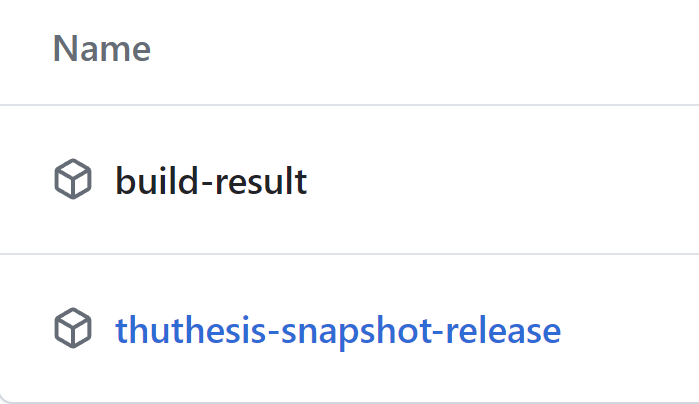
\includegraphics[height=.3\textheight]{thuthesis-download.png}
% \end{figure}
%     \end{column}
%   \end{columns}
% \end{frame}

\begin{frame}[fragile]{\ThuThesis 问题}
    \begin{itemize}
      \item 常见问题
        \begin{itemize}
          \item 参考文献列表出错、缺少字体、无法编译、格式不对……:先\textbf{更新到最新版本}试试
          \item 认真阅读文档 |thuthesis.pdf| 和使用示例 |thuthesis-example.pdf|
          \item 查看 FAQ \link{\ThuThesisLink/wiki/FAQ}
        \end{itemize}
      \item 主动提问
        \begin{itemize}
          \item GitHub Discussions 提问 \link{\ThuThesisLink/discussions}
          \item GitHub Issues 提交 bug \link{\ThuThesisLink/issues}
          % \item \TeX @newsmth 查找或发文
          % \item \ThuThesis{} Google Group 发问 \link{http://groups.google.com/group/thuthesis}
        \end{itemize}
    \end{itemize}
\end{frame}



%%% vim: set sw=2 isk+=\: et tw=80 cc=+1 formatoptions+=mM:

% !TeX encoding = UTF-8
% !TeX program = latexmk
% !TeX root = ../latex-talk.tex

\section{总结}

\printcurrenttoc

\begin{frame}{常见 \LaTeX{} 困惑}
  \begin{itemize}
    \item \alert{编译不通过} 缺少必要宏包,命令拼写错误,括号未配对等
    \item \alert{表格图片乱跑} 非问题,\LaTeX{} 浮动定位算法 \link{https://liam.page/2017/04/30/floats-in-LaTeX-the-positioning-algorithm/}
    \item \alert{段落间距变大} 非问题,\LaTeX{} 排版算法
  \end{itemize}
\end{frame}

\begin{frame}{系统学习}
  \begin{itemize}
      \item 《一份(不太)简短的~\LaTeXe{} 介绍》(lshort-zh-cn)~(1--2 天) \link{https://mirrors.tuna.tsinghua.edu.cn/CTAN/info/lshort/chinese/lshort-zh-cn.pdf}
      \item 包太雷 《\LaTeX{} Notes(第二版)》~(3小时)(lnotes2) \link{https://github.com/huangxg/lnotes}
      \item Stefan Kottwitz 《LaTeX Cookbook》
      \item WikiBooks:英文 \link{https://en.wikibooks.org/wiki/LaTeX}、中文 \link{https://zh.wikibooks.org/wiki/LaTeX}
      \item 在线教程:Overleaf 帮助文档 \link{https://www.overleaf.com/learn}
      \item 仔细阅读《\ThuThesis{} 用户手册》~(20 分钟)
      \item 从~\ThuThesis{} 示例文档入手修改
  \end{itemize}
\end{frame}

\begin{frame}{扩展阅读}
  \begin{itemize}
    \item 一份其实很短的 \LaTeX 入门文档 (Liam Huang) \link{https://liam.page/2014/09/08/latex-introduction/}
    \item \LaTeX{} 工作室:\url{https://www.latexstudio.net/}
    \item 知乎 \LaTeX{} 专栏(偏技术)\link{http://zhuanlan.zhihu.com/LaTeX}
    % \item \LaTeX{}杂谈(刘海洋)
    \item 《\LaTeX{}入门》(刘海洋)
    \item 现代 LaTeX 入门讲座(曾祥东)\link{https://github.com/stone-zeng/latex-talk/releases/tag/2019-04-18}
    \item “黑科技”:在 \LaTeX{} 中书写 Markdown 进行排版 \link{https://liam.page/2020/03/30/writing-manuscript-in-Markdown-and-typesetting-with-LaTeX/}
  \end{itemize}
\end{frame}


\begin{frame}[fragile]{利用文档}
  \begin{itemize}
    \item 常用文档
      \begin{itemize}
        \item \pkg{symbols}: 符号大全
        \item \pkg{Mathmode}: 数学参考
        \item \pkg{ctex}, \pkg{xeCJK}: 中文支持
        \item \pkg{texlive-zh}: \TL 安装与使用
        \item 所用宏包文档
      \end{itemize}
    \item 工具
      \begin{itemize}
        \item |tlmgr|: \TL 管理器
        \item |texdoc|: \TeX{} 文档查看器\\
          例如:|texdoc lshort-zh-cn|
        \item 在线文档 \TeX{}doc \link{http://texdoc.net/}
        \item TeX Studio 和 WinEdt 都支持在帮助里看文档
      \end{itemize}
  \end{itemize}
\end{frame}

\begin{frame}{一点人生的经验}
  \begin{itemize}
    \item 不要着急安装,先在 Overleaf 上熟悉各类操作
    \item 不要过于相信网上的中文教程/博客等
      \begin{itemize}
        \item 简单鉴别方法: 排版的好看程度
      \end{itemize}
    \item 实验室祖传的 \CTeX{} 套装多半是过时的,\ThuThesis{} 八成是老版本的
    \item 如果你要处理中文:
      \begin{itemize}
        \item \textbf{使用 \XeLaTeX{}},使用 \XeLaTeX{},使用 \XeLaTeX{}
        \item \textbf{忘记 \pkg{CJK}},忘记 \pkg{CJK},忘记 \pkg{CJK}
        \item 使用 \pkg{ctex} 宏包(2.0以上版本)(跟 \CTeX{} 套装仅仅是名字像)
      \end{itemize}
    \item 写一点,编译一次,减小排错搜索空间
  \end{itemize}
\end{frame}

\begin{frame}[fragile]
  \frametitle{Git版本管理}
  \begin{itemize}
    \item 版本管理的必要性
      \begin{itemize}
        \item 远离「初稿,第二稿……终稿,终稿(打死也不改了)」命名
        \item 方便与他人协同合作
      \end{itemize}
    \item 基本用法
      \begin{itemize}
        \item 跟踪更改:|git init|、|git add|、|git commit|
        \item 撤销与回滚:|git reset|、|git revert|
        \item 分支与高级用法:|git branch|、|git checkout|、|git rebase|
        \item 远端仓库操作:|git pull|、|git push|、|git fetch|
        \item 推荐用 VS Code 等进行可视化操作
        \item 参考链接:\link{https://git-scm.com/book/en/v2}
          \link{https://www.liaoxuefeng.com/wiki/0013739516305929606dd18361248578c67b8067c8c017b000}
      \end{itemize}
    \item 在线 Git 服务
      \begin{itemize}
        \item GitHub \href{https://github.com}{\faGithub}
        \item 清华大学代码托管服务(基于 GitLab) \link{https://git.tsinghua.edu.cn}
      \end{itemize}
  \end{itemize}
  \end{frame}

% 寻求帮助
\begin{frame}{寻求帮助}
  \begin{columns}[c]
    \begin{column}{.45\textwidth}
      \begin{itemize}
        \item BBS
          \begin{itemize}
            \item 水木社区 TeX 版 (不活跃)\link{http://www.newsmth.net/nForum/board/TeX}
            \item GitHub 上的 \CTeX 社区 \link{https://github.com/CTeX-org/forum}
          \end{itemize}
        \item UK FAQ \link{http://www.tex.ac.uk/cgi-bin/texfaq2html}
        \item \TeX{} StackExchange \link{https://tex.stackexchange.com/}
        \item Google, Bing, etc.
          \begin{itemize}
            \item 使用\textbf{英语}搜索
          \end{itemize}
        \item 大语言模型(LLM)助手......?
      \end{itemize}
    \end{column}
    \begin{column}{.45\textwidth}
      
\includegraphics[width=\textwidth]{TFZsuperellipse-crop.png}
    \end{column}
  \end{columns}
\end{frame}

\begin{frame}{相关工具}
  万变不离其宗,掌握 \LaTeX{} 后,可尝试不同工具适应自身需要、提高排版效率:
  \begin{itemize}
    \item 基于 \TeX{} 生态的辅助工具:
    \begin{itemize}
      \item Texifier \link{https://www.texifier.com/}(商业软件,仅 Apple 平台,原名 Texpad):实时生成 \LaTeX{} 项目的 PDF 编译结果
      \item LyX \link{https://www.lyx.org/}(自由软件):所见即所得,使用 \TeX{} 语法,但部分功能受限
      \item Tectonic \link{https://tectonic-typesetting.github.io/}(自由软件):Rust 编写的、基于 \XeTeX{} 的现代 \LaTeX{} 引擎,编译速度快、安装体积小
    \end{itemize}
    \item 类 \TeX{} 的文档排版软件:
    \begin{itemize}
      \item GNU TeXmacs \link{https://zh.wikipedia.org/zh-cn/GNU_TeXmacs}(自由软件):所见即所得,可转换为 \TeX{} 代码输出
      \item typst \link{https://typst.com/}(自由软件):新兴的使用 Rust 编写的排版系统,支持结构化语法、排版速度快、社区活跃,但生态尚待完善
    \end{itemize}
  \end{itemize}
\end{frame}

\begin{frame}{你也可以帮助}
  \begin{itemize}
    \item 错误反馈、改进建议:GitHub Issues \link{https://github.com/tuna/thulib-latex-talk/issues}
    \item 出力维护:\LaTeX{} 宏包、模板编写,bug 修复
    \item 科普、答疑 
    \item \sout{来当主讲人}
  \end{itemize}
\end{frame}

%%% vim: set ts=2 sts=2 sw=2 isk+=\: et tw=80 cc=+1 formatoptions+=mM:


\begin{frame}
  \begin{center}
    {\Huge\calligra Thank you!} %\\[0.5em]
    % 烦请填写调查问卷(请稍后查看雨课堂公告)\\
    % \url{\surveylink} \\[1em]
    % \qrcode[hyperlink, height=3.5cm]{\surveylink}
  \end{center}
\end{frame}

\end{document}

%%% vim: set ts=2 sts=2 sw=2 isk+=\: et tw=80 cc=+1 formatoptions+=mM:
